This paper considers the following learning task. Suppose we have a set of items
along with human-judged pairwise similarities among them. For example, the
items could be visual stimuli such as advertisements, pictures, or diagrams.
Assume that we also have a high-dimensional feature associated with each item.
The learning task is to determine which of the many features are most predictive
of the perceptual similarities. This can be posed mathematically as follows.
Let $\bS$ be an $n\times n$ matrix of pairwise similarities between $n$ items.
Let $\bX$ be an $n\times p$ matrix where the $i$th row is the $1\times p$ vector
of the features for item $i$. Then we wish to find a weight matrix $\bW$ such
$\bX\bW\bX^T \approx \bS$. The structure of the weight matrix reveals which
features are most important in representing the perceptual similarities. We call
this {\em Representational Similarity Learning}.

Let us illustrate this problem with two applications. First, suppose the
representations are molecular diagrams used to train chemistry students. We
gather visual pairwise similarity judgments about the diagrams from the
students. We also have a feature for each diagram (e.g., counts of different
atom types, counts of bounds, bound angles, etc). The goal is to determine
which features are driving the visual similarity judgments of the students.
Second, consider {\em Representational Similarity Analysis} (RSA) in fMRI brain
imaging ~\cite{RSA}. In RSA a person is scanned while viewing $n$ different
visual stimuli. Pairwise similarities are obtained through other experiments,
such as asking people to look at pairs of stimuli and rate the similarity. In
this case, the features are the stimuli responses of $p$ voxels in the brain,
and the goal is to determine which voxels (and hence brain regions) are encoding
the similarities. RSA is depicted in Figure~\ref{Fig.WRSA}, and it is the focus
of our application in Section~\ref{sec:rsa}.
\begin{figure}[!h]
	\centering
    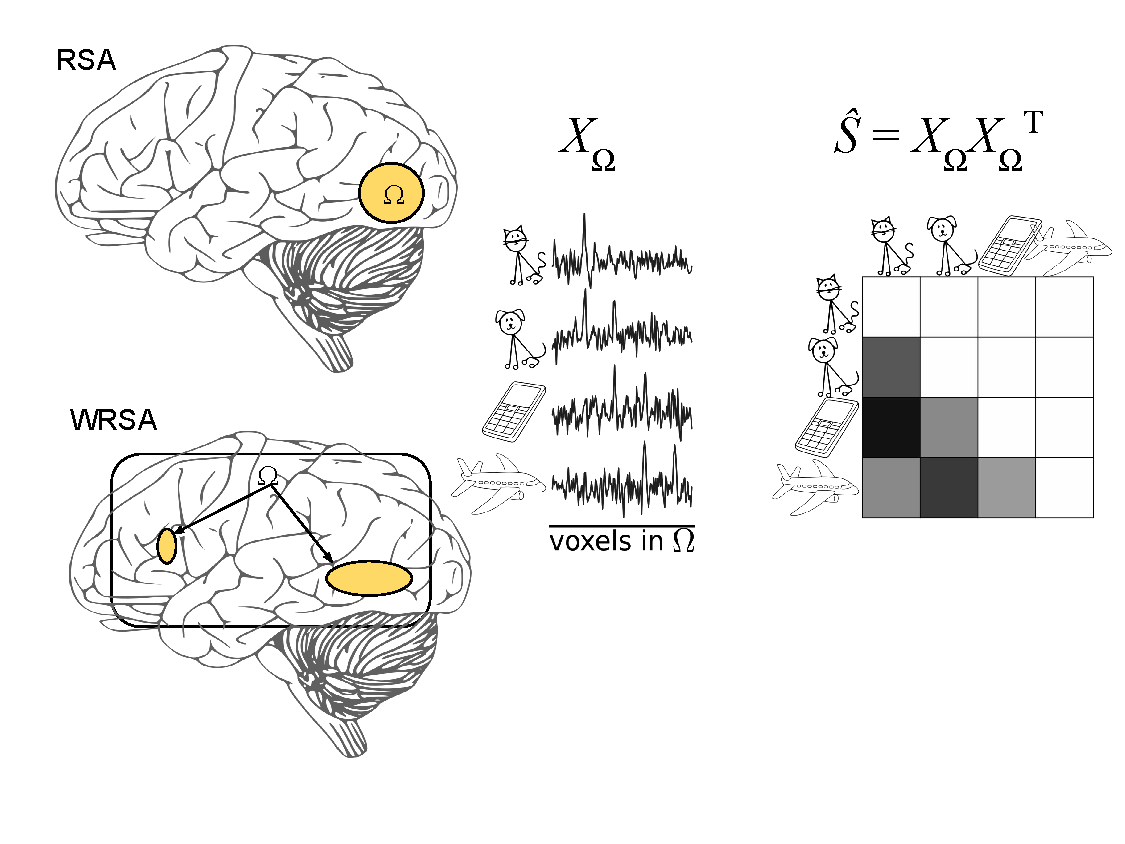
\includegraphics[width=0.5\textwidth]{figures/WRSA.pdf}
    \caption{Representational Similarity Analysis. Traditional RSA methods
      consider only localized brain regions of interest or spherical clusters in
      the cortex (upper left)~\cite{RSA,searchlight}. In Section~\ref{sec:rsa},
      we propose a new {\em Network} RSA (NRSA) method that can potentially
      identify non-local brain networks that encode similarity information
      (lower left). }
    \label{Fig:WRSA}
\end{figure}

\subsection{Representational Similarity Learning}

Let $\bX \in \R^{n\times p}$ denote a feature matrix. Each row corresponds to
$p$ features associated with a specific item, and each column corresponds to the
values of a specific feature for each of the $n$ items. The goal of RSL is to
find a sparse and symmetric matrix $\bW\in \R^{p\times p}$ such that

$$\bS \ \approx \bX \bW \bX^T \ .$$

By sparse we mean that at most $k<p$ rows/columns of $\bW$ are nonzero. The
locations of the nonzero elements indicate which features are included in the
similarity representation. For instance, consider the $n\times 1$ vectors
corresponding features $\bx_k$ and $\bx_{\ell}$ (i.e., the $k$th and $\ell$th
columns of $\bX$). It is easy to show that the contribution of these two
features to the similarity representation is given by $ W_{k,\ell} \, \bx_k
\bx_{\ell}^T + W_{\ell,k} \, \bx_\ell \bx_{k}^T$. If $W_{k,\ell}=W_{\ell,k}\neq
0$, then the correlations between the two features contribute to the
approximation of the similarity matrix $\bS$. The complete similarity
representation can be expressed as

$$\bS \ \approx \ \bX\bW\bX^T \ = \ \sum_{k,\ell=1}^p W_{k,\ell} \, \bx_k \bx_{\ell}^T \ .$$

The approximation problem can be posed as the least squares optimization

$$\min_{\bW} \|\bS-\bX\bW\bX^T\|_F^2 \ , $$

where the objective is the Frobenius norm of the difference between the
similarity matrix $\bS$ and its approximation in terms of voxel activations.
Suppose $\bS$ is a positive semi-definite matrix, then there exists a matrix
$\bY$ which satisfies $\bS=\bY\bY^T$ (e.g., obtained via eigendecomposition or
Cholesky decomposition). Thus, we may instead consider the optimization

$$\min_{\bB} \|\bY-\bX\bB\|_F^2 \ . $$

For any coefficient matrix $\bB$ the corresponding weight matrix is given by
$\bW = \bB\bB^T$. Both optimizations are convex, but we will work with the
latter since it tends to be easier to solve and also allows us to easily
incorporate constraints or regularizers. Note that, for the sake of simplicity,
we only focus on PSD matrices here; the corresponding argument for other
matrices is described in the supplementary material.

The weight matrix $\bW$ and the coefficient matrix $\bB$ are often expected to
exhibit sparsity and low-rank structure. Indeed, our hypothesis is that a small
subset of the features encodes the similarity representations, hence the
sparsity. Similarity matrices are often low-rank because of clustering or other
relationships between the items under consideration. For example, in our fMRI
application described later in the paper, we find that a rank $r=3$
approximation is quite accurate. We also expect $\bW$ and $\bB$ to be low-rank
because of clustering relationships between the features. To account for this,
the optimization above can be modified to obtain sparse and low-rank solutions,
as described next.

\section{Representational Similarity Learning via Group Lasso}

Consider the group lasso optimization
\begin{equation}\label{eqn.grouplasso}
 \min_{\bB\in \R^{p\times r}} \|\bY-\bX\bB\|_F^2 \ + \ \lambda \|\bB\|_{1,2} \ .
\end{equation}

Note that the optimization variable $\bB$ is a $p\times r$ matrix, which
guarantees a rank $r$ (or less) solution, and thus similarity representation
$\bX\bB\bB^T\bX^T$ will be rank $r$ at most, which is a simple way to enforce
the low-rank constraint. The parameter
$\lambda>0$ is an adjustable weight on the sparsity-promoting regularizer
$\|\bB\|_{1,2}$, which is defined as follows. The rows of $\bB$ are denoted by
$\bbeta_{i\a}$, $i=1,\dots,p$, and the norm
$\|\bB\|_{1,2} \ = \ \sum_{i=1}^p \|\bbeta_{i\a}\|_2$.
This encourages solutions with only a few nonzero rows in $\bB$
\citep{obo11,lounici,vandegeer}.

The main technical innovation in this paper is a new approach to the group lasso
that is designed to cope with strongly correlated covariates (\ie cases in which
certain columns of $\bX$ may be close to, or even exactly, collinear). This is a
concern in fMRI, since certain voxels may have very correlated activation
patterns. This problem is illustrated in Figure~\ref{Fig:sim}, where we simulate
a situation where columns $5$ and $7$ of the data matrix $\bX$ are highly
correlated. Group lasso selects one of the corresponding rows in $\bB$ (row
$5$), whereas GrOWL correctly selects both rows $5$ and $7$.

\begin{figure}[!h]
  \centering
    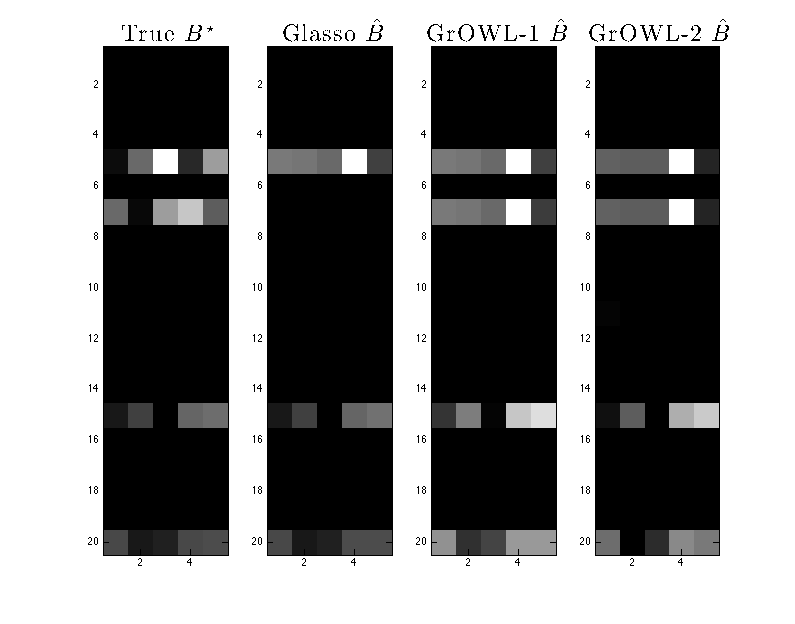
\includegraphics[width=0.5\linewidth]{sim3.png}
    \qquad
    \caption{A comparison of group lasso (middle) and grOWL (right) optimization
      solutions with correlated columns in $\bX$ showing that GrOWL selects
      relevant features (row 5 and 7) even if they happen to be strongly
      correlated and automatically cluster them by setting the corresponding
      coefficient rows to be equal (or nearly equal).}
    \label{Fig:sim}
\end{figure}

In the standard (single-task) regression problem, this issue has been tackled
using many techniques, including the elastic net \cite{EN}, OSCAR \cite{oscar}
and OWL \cite{owl}, and others. We propose a generalization of the recently
proposed Ordered Weighted $\ell_1$ (OWL) approach to the multi-task setting, and
thus call our new approach Group OWL (GrOWL). We show that GrOWL shares many of
the desirable features of the OWL method, namely it automatically clusters and
averages regression coefficients associated with strongly correlated columns of
$\bX$. This has two desirable effects, in terms of both model selection and
prediction. First, GrOWL can select all of the relevant voxels in $\bX$, unlike
standard group lasso which may not select relevant voxels if they happen to be
strongly correlated with others. Second, GrOWL encourages the coefficients
associated with strongly correlated voxels to be near or exactly equal. In
effect, this averages strongly correlated voxels which can help to denoise
activation patterns and improve predictions.
